\chapter{Metodologia}
\label{cap:metodologia}

[Descreva o tipo de pesquisa, os materiais, os métodos e as etapas do trabalho.]

\section{Figuras}

% Ilustrações (NBR 14724, 5.8, e template UFERSA):
%  - título acima, precedido da palavra "Figura", do número e de travessão;
%  - fonte abaixo, em tamanho menor (obrigatória, mesmo que seja produção
%    do próprio autor);
%  - a ilustração deve ser citada no texto e inserida o mais próximo
%    possível do trecho a que se refere.
% O minipage alinha o título e a fonte às bordas da figura.

A Figura~\ref{fig:exemplo} apresenta um exemplo de ilustração.

\begin{figure}[htbp]
	\centering
	\begin{minipage}{0.6\textwidth}
		\caption{Exemplo de figura}
		\label{fig:exemplo}
		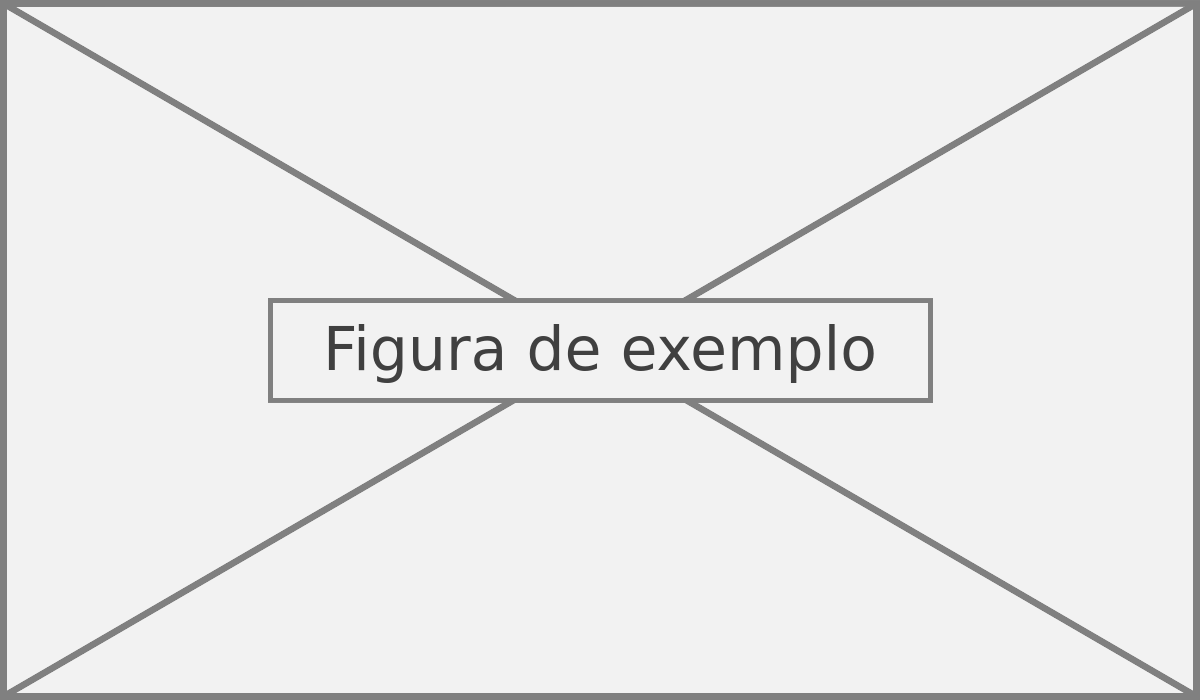
\includegraphics[width=\linewidth]{figuras/exemplo-figura}
		\Fonte{Elaborada pelo autor ([Ano]).}
	\end{minipage}
\end{figure}

\section{Quadros}

% Quadros: conteúdo textual/qualitativo, com bordas fechadas.

O Quadro~\ref{qua:exemplo} apresenta um exemplo de quadro.

\begin{quadro}[htbp]
	\IBGEtab{%
		\caption{Exemplo de quadro}
		\label{qua:exemplo}
	}{%
		\begin{tabular}{|p{4cm}|p{8cm}|}
			\hline
			\textbf{Elemento} & \textbf{Descrição} \\
			\hline
			[Elemento 1] & [Descrição do elemento 1] \\
			\hline
			[Elemento 2] & [Descrição do elemento 2] \\
			\hline
		\end{tabular}%
	}{%
		\Fonte{Elaborado pelo autor ([Ano]).}%
	}
\end{quadro}
